\chapter{Related work}
\label{c:relatedwork}

\todo[inline]{Introductory Paragraph}
\todo[inline]{Structuring}

\begin{figure}[b]
	\centering
	
	\begin{subfigure}[b]{0.45\textwidth}
		\centering
        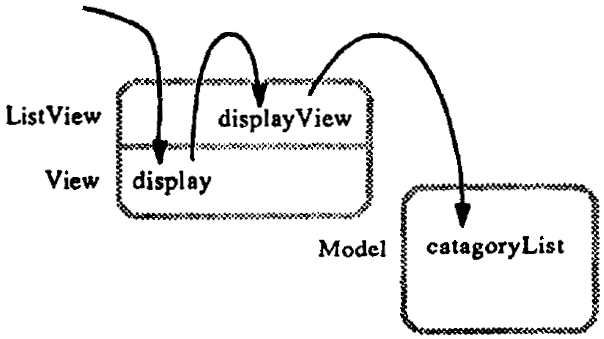
\includegraphics[width=\textwidth]{../images/06-Cunningham-Diagram}
        \caption[Object Interaction Diagrams by Cunningham and Beck]{}
		\label{fig:06-1-Cunningham}
	\end{subfigure}
	\quad
	\begin{subfigure}[b]{0.45\textwidth}
		\centering
		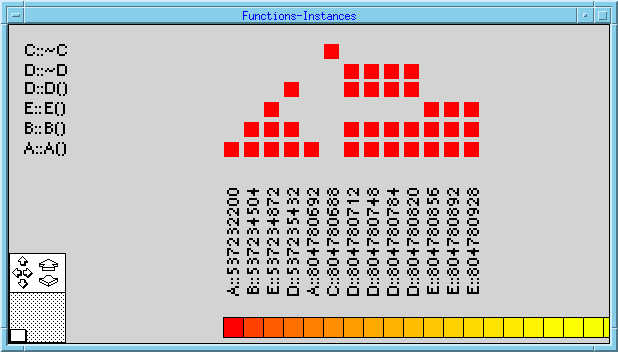
\includegraphics[width=\textwidth]{../images/06-DePauw-Matrix}
		\caption[Functions-Instances Matrix by De Pauw et al.]{}
		\label{fig:06-1-DePauw}
	\end{subfigure}
	
	\caption[TOC Caption]{
		a) Cunningham's and Beck's notion of diagramming object interactions, taken from \cite{cunningham_diagram_1986}.
		b) Functions-Instances Matrix by De Pauw et al., adapted from \cite{de_pauw_visualizing_1993}.
	}
	\label{fig:06-1}
\end{figure}

Cunningham and Beck propose a syntax for diagramming the message sending dialogue between objects in object-oriented computations (see Figure \ref{fig:06-1-Cunningham}) \cite{cunningham_diagram_1986, beck_system_1989}.
Similar to \textsc{PathObjects}, objects are drawn as boxes and message sends are represented by directed arcs between them.
Unlike the notation used by \textsc{PathObjects}, the space inside the boxes is not used to model the object state, but to emphasize method overrides and calls to implementations of superclasses.
For that purpose, the class hierarchy is represented by layers in a box.
Since the authors regard overriding as the more important concept over inheritance, subclasses are placed above superclasses in these layers. 
To allow for the generation of such diagrams, an additional pane is added to the Smalltalk-80 debugger. 
Objects and messages are added to this diagram area when using the standard debugger commands \emph{step} and \emph{send}. 
However, as automatic layouting is not supported, objects have to be placed by the user manually. 
The authors state that the debugger extension helped them to understand complicated computations better, enabling them to fix a long standing bug in the Smalltalk core.

De Pauw et al. present a number of object-oriented views \cite{de_pauw_visualizing_1993, tokoro_modeling_1994} that can be generated and updated either live during the execution of instrumented code or post-mortem from recorded execution traces.
In our context of object interactions, the \emph{Functions-Instances Matrix} view  which shows the number of calls of specific methods on specific instances (cf. Figure \ref{fig:06-1-DePauw}) is of particular interest.
Methods are drawn on the y axis and instances are shown on the x axis.
Each box in the matrix denotes a call of the method from the left on the object at the bottom.
The color of the box indicates the number of invocations.
Although the diagram doesn't show object interactions in the presented form, it could be easily extended in this sense by replacing the static information on the y axis that abstracts from concrete instances through corresponding representations.
However, this matrix can not be utilized to visualize a specific sequence of function invocations or the state of the instances, both of which are important concepts of \textsc{PathObjects}.
The other presented views mainly focus on classes and their relationships, but an adaption to a visualization at the abstraction level of objects is straightforward in most cases.

\textsc{Scene} by Koskimies and Mössenböck \cite{koskimies_scene:_1996} provides interactive visualizations of Oberon programs in the form of scenario diagrams.
Execution traces from instrumented program runs serve as a basis, whereby the instrumentation can be conducted at the granularity of Oberon modules.
Just like in UML sequence diagrams, objects are represented by vertical lines, and interactions between those objects are represented by horizontal arrows.
To deal with the problem of large traces and limited screen  real estate, the authors propose \emph{call compression} and \emph{partitioning}.
Call compression means that all message sends are collapsed initially and can be expanded by the user through clicking on them.
Partitioning is employed since the authors consider vertical scrolling as acceptable, but want to avoid horizontal scrolling. Thus, if the size of the diagram exceeds the horizontal viewport, a new window is opened and the visualization is continued there.
\textsc{Scene} also allows the user to inspect the state of an object before and after a method invocation.
However, contrary to our approach which displays the actual state of objects and allows the user to explore complex referenced objects, this feature only utilizes user-provided \emph{Print} methods every object is supposed to have and displays static print strings.
\textsc{Scene} also does not offer ways to filter a trace by methods or classes or to search for specific entities of interest.

Lange and Nakamura present \textsc{Program Explorer} in the context of design pattern based framework understanding \cite{lange_interactive_1995, lange_program_1995}.
Based on the assumption that the combination of abstract concepts like classes and their relationships and the concrete objects and their interactions is the fundamental requirement to the understanding of object oriented systems, \textsc{Program Explorer} offers class inheritance views, object graphs and interaction charts.
Contrary to our approach, object state exploration is not supported.
To ensure a certain degree of scalability of the information presentation, \emph{view navigation} and \emph{integration} are provided.
Within a given view, \emph{navigation} can be used to explore the presented information interactively, starting from an initial focus point and going to regions of further interest.
\emph{Integration} enables the user to transfer a defined focus between different views.
Both concepts are similar to the navigation through a scenario offered by \textsc{PathObjects} and the bidirectional connection to the static view provided by \textsc{PathView}.
To reduce the size of the traces that are generated from instrumented executions of C++ programs, \textsc{Program Explorer} also supports \emph{trace localization}, which means that classes of interest can be selected through the instrumentation GUI and only selected classes will be instrumented.
As compared to \textsc{PathObjects}, the latter offers a more fine-grained approach through the selection of methods of interest, instead of solely filtering by classes.

The unique feature of \textsc{ISVis} \cite{jerding_using_1997} that also presents object interactions in the form of sequence diagram-like scenario views is the concept of \emph{ information murals} \cite{jerding_information_1998, jerding_visualizing_1996}.
The target of this approach is to provide a miniature view of large execution traces as a whole (cf. Figure \ref{fig:06-2-Mural}).
Classes are represented by rows on the vertical axis and a message between objects of different classes is drawn as a vertical line between the respective rows.
Users can assign colors to classes of special interest, which leads to an emphasis of the corresponding messages.
The horizontal axis represents time.
To avoid over-plotting, Visual properties like gray-scale shading or color intensity are exploited to map multiple elements to a single pixel or column.
Thus, the visual properties an original visualization would have if it could be viewed in its entirety are supposed to be preserved as effectively as possible.
Jerding et al. state that this view enables the user to find interaction patterns in large execution traces, which again helps in identifying usage scenarios and program components.

\begin{figure}[tb]
	\centering
	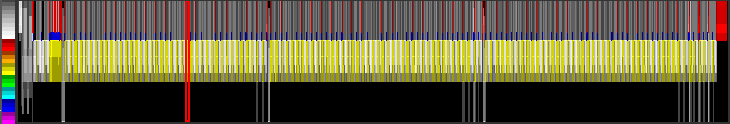
\includegraphics[width=0.8\textwidth]{../images/06-Mural}
	\caption[Information Mural by Jerding et al.]{Information mural displaying the execution of a bubble-sort algorithm with over 90,000 messages between 200 classes (adapted from \cite{jerding_information_1998}).}
	\label{fig:06-2-Mural}
\end{figure}


\textsc{JAVAVIS} by Oechsle and Schmitt \cite{diehl_javavis:_2002} was designed to aid in the teaching of the object oriented programming concepts of the Java environment.
It utilizes the Java Debug Interface to retrieve run-time information and can be used to step through the execution of a program.
Two main views are offered.
First, an UML sequence diagram is used to display the function call history of the current execution which grows successively as the user steps through the program.
Second, an UML object diagram is generated for each active invocation on all call stacks of the program under investigation.
These diagrams display the state of the receiving object, of local variables, and of the method's arguments.
That means that contrary to the approach implemented by \textsc{PathObjects}, object state and communication between objects are presented in different views.
The choice of using JDI debug sessions as data source implies further restrictions.
Only those objects that are currently present on the call stack can be inspected, while our solution also allows the user to explore the state of objects that have been used in the past but are not involved in the computation that is displayed.
Furthermore, a search for object or method occurrences is not possible for the future execution, and also not offered for the execution history.
The same applies to the unrestricted navigation to specific points of the execution.

\textsc{Collaboration Browser} by Richner and Ducasse \cite{richner_using_2002} is a tool that focuses on the recovery of object collaborations and roles from dynamic information.
Since the process of automatic design recovery is said to yield poor results, the authors favor an iterative process steered by an engineer.
To facilitate such a process, \textsc{Collaboration Browser} offers two main features: \emph{pattern matching} and \emph{querying}. 
Typically, a user would first create collaboration patterns by defining pattern matching criteria, and then proceed by iteratively querying about patterns in which classes or methods of interest participate.
Finally, to understand a collaboration, an instance of a collaboration pattern can be visualized in the form of interaction diagrams, which are almost identical to UML sequence diagrams. \todo{compare to PathObjects}

Systä et al. present a reverse engineering environment called \textsc{Shimba} \cite{systa_shimba_2001}, which supports both static and dynamic analysis of Java software systems.
Static information about software entities like classes, interfaces and their relationships is extracted from the bytecode representation and visualized using \textsc{Rigi} \cite{muller_understanding_1993} in the form of directed dependency graphs.
Besides the computation of some of the metrics of Chidamber's and Kemerer's suite \cite{chidamber_metrics_1994}, \textsc{Rigi} also can be utilized to build abstractions, for instance by aggregating classes into their respective packages.
Runtime traces are collected with the help of a customized SDK debugger and can be synthesized as UML-like sequence and statechart diagrams through \textsc{SCED} \cite{koskimies_automated_1998,systa_understanding_2000}.
\textsc{Shimba} supports bidirectional model slicing between \textsc{Rigi} graphs and \textsc{SCED} diagrams.
On one side, \textsc{Rigi} can be used to restrict the amount of collected execution events through the selection of components of interest. Thus, the scope of the generated \textsc{SCED} diagrams is reduced.
On the other side, starting from a \textsc{SCED} diagram, static views covering the affected components can be obtained.